\section{Scenario Services}
\label{ch:scenarios}

\ac{Luci} uses GeoJSON format to represent scenario geometry.
The format declares geometry information syntax, but does not declare consistent naming and geometry type mappings for \ac{Luci} scenario entities, such as buildings, roads, etc.
This document aims at providing guidelines on usage of \ac{Luci} scenarios in \ac{Luci} clients and services.

\paragraph{A note on jsonGeometry data type}
The word \texttt{geometry} in \ac{Luci} specification has two different meanings.
On the one hand it is a name of the key that occurs from time to time in \ac{Luci} actions.
On the other hand it is a name of a pre-defined data type that represents scenario geometry in JSON format.
To resolve this ambiguity, in current document we use word \texttt{geometry} to represent the name of the key, and \texttt{\color{blue}jsonGeometry} to represent the data type.
This differentiation does not introduce any changes to the existing JSON messages.

\subsection{\acs{Luci} scenario actions}
\label{ch:scenarios:actions}

% {"name":"shp_file_test","action":"create_scenario","geometry":{"anl.dbf":{"format":"dbf","attributeMap":{"geomid":"objectid","timestampformat":"YYYY","timestamp":"yearofchan"},"streaminfo":{"checksum":"48AC6C5CD751A525778A144EB66727","length":3138,"order":2}},"anl.shp":{"format":"shp","streaminfo":{"checksum":"39FBD5108DED0FF5637721A4820C484","length":1444,"order":1}},"anl.shx":{"format":"shx","streaminfo":{"checksum":"6B6F93D87FB73FF1AB92C3BD2938D2C","length":484,"order":3}}}}

To send geometry to \ac{Luci}, we wrap it in the structure that is shown in listing~\ref{json:geometry}
Special type \texttt{\color{blue}jsonGeometry} wraps various types of geometry processed by \ac{Luci}.
It allows to enclose arbitrary number of custom-named geometries (keys \texttt{KEY\_NAME\_N}) inline (GeoJSON) or in separate files (as binary attachments).
%
\begin{lstlisting}[caption={structure of \texttt{\color{blue}jsonGeometry} data type}, label={json:geometry}]
{
	/* key name is an arbitrary string.
	   The convention is to name it by filename of a file,
	   or arbitraryname.geojson in case of GeoJSON geometry */
	KEY_NAME_1 :
		XOR { // "in-line" geometry
			format   : string // "GeoJSON", later add also TopoJSON, CurveJSON, ...
			geometry : object // GeoJSON FeatureCollection
			OPT crs  : string // name of a crs
			OPT attributeMap : { // mapping between Luci and foreign types
				LUCI_ATTRIBUTE_NAME : FOREIGN_ATTRIBUTE_NAME,
				...
			}
		}
		XOR { // "streaminfo" - attachment description
			format     : string // shp | shx | dbf | any other file format?
			streaminfo : {
				checksum : string // MD5 sum of an attached binary data
				length : long // length of the attached binary data
				order : long // number of attachment (starts with 1)
			}
			OPT crs    : string // name of a crs
			OPT attributeMap : { // mapping between Luci and foreign types
				LUCI_ATTRIBUTE_NAME : FOREIGN_ATTRIBUTE_NAME,
				...
			}
		},
	KEY_NAME_2 : ...,
	...
}
\end{lstlisting}
%
The type of object \texttt{geometry} is GeoJSON \texttt{FeatureCollection} -- the format that is described in GeoJSON specification\footnote{\url{http://geojson.org/geojson-spec.html}}.


%Note, according to \ac{Luci} specification, object \texttt{geometry} is exchangeable (\texttt{XOR}) with \texttt{streaminfo}; however, no examples of \texttt{streaminfo} are provided, so \texttt{streaminfo} is excluded from this document.
%Also file \path{spec/luci_spec_todo.pdf} shows the format a bit more clear (geojson vs streaminfo), but I am not sure which version is implemented right now in Luci.
%\comment{This is a question to Lukas. }

According to \path{spec/LuciSpecification.pdf},
\ac{Luci} provides three operations to work with scenarios:
\texttt{create\_scenario}, \texttt{update\_scenario}, and \texttt{get\_scenario}.
This document covers only GeoJSON geometry manipulation;
in this format individual entities are represented as \texttt{Feature} objects in \texttt{FeatureCollection}.
Each \texttt{Feature} has a property \texttt{geomID:\color{blue}long} that is given either by a client, or by \ac{Luci} (in case if client application does not specify property \texttt{geomID}).


Creating a scenario is done
via \texttt{create\_scenario} action shown in listing~\ref{action:createScenario}.
The action allows to specify a location (\texttt{projection}) and a geometry to put inside the new scenario.
\begin{lstlisting}[caption={JSON action structure for creating a scenario in \ac{Luci}}, label={action:createScenario}]
{
	action           : "create_scenario", // constant, represents the action
	name             : string, // name of the scenario
	OPT projection   : {
		XOR crs    : string, // name of a crs
		XOR bbox   : [ [number, number]   // top-left coords [lat, long]
		             , [number, number]], // bottom-right coords [lat, long]
	},
	OPT geometry     : jsonGeometry, // wrapper around various geometry types
	OPT switchLatLon : boolean // switch lat-long to long-lat in geometry
}
\end{lstlisting}


Listing~\ref{action:updateScenario} shows the action to update scenario geometry.
The action allows to change the name and the bounding box, as well as the geometry inside.
\begin{lstlisting}[caption={JSON action structure for updating a scenario in \ac{Luci}}, label={action:updateScenario}]
{
	action       : "update_scenario", // constant, represents the action
	ScID         : long, // ID of the scenario in Luci
	OPT name     : string, // set a new name for the scenario
	OPT bbox     : [ [number, number]   // top-left coords [lat, long]
	               , [number, number]], // bottom-right coords [lat, long]
	OPT geometry : jsonGeometry // wrapper around various geometry types
	OPT switchLatLon : boolean // switch lat-long to long-lat in geometry
}
\end{lstlisting}
\begin{itemize}
\item In order to add an entity to the scenario, one adds \texttt{Feature} into \texttt{FeatureCollection} (\texttt{geometry} object).
\item In order to modify an existing entity, one must specify its property \texttt{geomID} (if given \texttt{geomID} does not exist, the entity is added to the scenario, otherwise it is edited).
\item In order to delete a number of entities from the scenario, one adds an empty \texttt{Feature} into \texttt{FeatureCollection} that has a property \texttt{deleted\_geomIDs:[\color{blue}long\color{black}]} -- array of \texttt{geomID} for deletion.
\end{itemize}

Listing~\ref{action:getScenario} shows the action to get scenario geometry.
The action allows to specify the format of the data to (\ac{Luci} does transformation),
and get the geometry from the scenario at given time.
\begin{lstlisting}[caption={JSON action structure for getting a scenario from \ac{Luci}}, label={action:getScenario}]
{
	action             : "get_scenario", // constant, represents the action
	XOR scenarioname   : string // name of the scenario in Luci
	XOR ScID           : long, // ID of the scenario in Luci
	OPT format_request : string, // maybe we will change this later to "format"
	OPT crs            : string,
	OPT geomIDs        : [long], // select a subset of scenario objects
	OPT timerange      : { // time is a number - timestamp in unix format
		XOR until   : long,
		XOR from    : long,
		XOR between : [long,long],
		XOR exactly : long,
		OPT all     : boolean // include all versions (not only the last)
	}
}
\end{lstlisting}

\subsection{Scenario GeoJSON geometry}
\label{sec:services:scenario}

Although GeoJSON specification provides all necessary geometry primitives,
we need a more structured convention to define one-to-one mapping between the geometry and scenario entities.
\ac{Luci} does not generate an error for an input that does not follow it -- the convention only describes what kind of data structures services and clients should expect.

Section~\ref{ch:scenarios:standardrules} describes the rules assumed by \ac{Luci} when communicating with all services and clients.
Section~\ref{ch:scenarios:conventionalrules} describes the rules assumed by most applications, but not checked in \ac{Luci}.
Section~\ref{ch:scenarios:applicationrules} describes the application-specific rules.
Any service or client provider (\ac{Luci} user) may introduce a rule that is used in their application.
The providers are encouraged to add these rules into section~\ref{ch:scenarios:applicationrules}.
By an agreement in our team some of the rules go up from section~\ref{ch:scenarios:applicationrules} to section~\ref{ch:scenarios:conventionalrules}.
In case of wide usage they might be enforced in \ac{Luci}, thus moving one step up to section~\ref{ch:scenarios:standardrules}.

\subsubsection{Standardized Rules}
\label{ch:scenarios:standardrules}
Object \texttt{geometry} in listing~\ref{json:geometry} is assumed to be of type \texttt{FeatureCollection}.
Every entity is represented as a \texttt{Feature} inside that collection, and has a property \texttt{geomID:\color{blue}long} that is given by a client or \ac{Luci} (if the client omits the property).

\subsubsection{Conventional Rules}
\label{ch:scenarios:conventionalrules}

Some services require 3D objects, others use only 2D footprints.
To distinguish these two types of geometry, we agreed on using \texttt{Feature} property \texttt{layer}.
\begin{itemize}
\item Object (e.g. Building) -- a 3D geometry, represented as \texttt{Feature} with \texttt{geometry} field of type \texttt{Polygon} or \texttt{MultiPolygon}.
To be processed correctly by \ac{Luci} services, the object requires property \texttt{layer:\color{red}"buildings"}.
%
\item Footprint -- a 2D geometry, represented as \texttt{Feature} with \texttt{geometry}
field of type \texttt{Polygon} or \texttt{MultiPolygon}.
To be processed correctly by \ac{Luci} services, the footprint requires property \texttt{layer:\color{red}"footprints"}.
\end{itemize}


\subsubsection{Per-application Rules}
\label{ch:scenarios:applicationrules}

\paragraph{Web geometry modeler}
The application distinguishes dynamic and static geometry:
dynamic geometry can be edited, static geometry is only used for evaluation and visualization.
Thus, I propose an optional property \texttt{static:\color{blue}boolean}.
Absence of a property implies \texttt{static:\color{brown}false}.

\subsubsection{Example for Scenario Usage}
\label{ch:scenarios:example}
The following example illustrates a service registering to Luci and being subsequently called by a client. The service queries a scenario from the scenario service and returns some analysis result to the client.
\begin{figure}[h!]
	\centering
	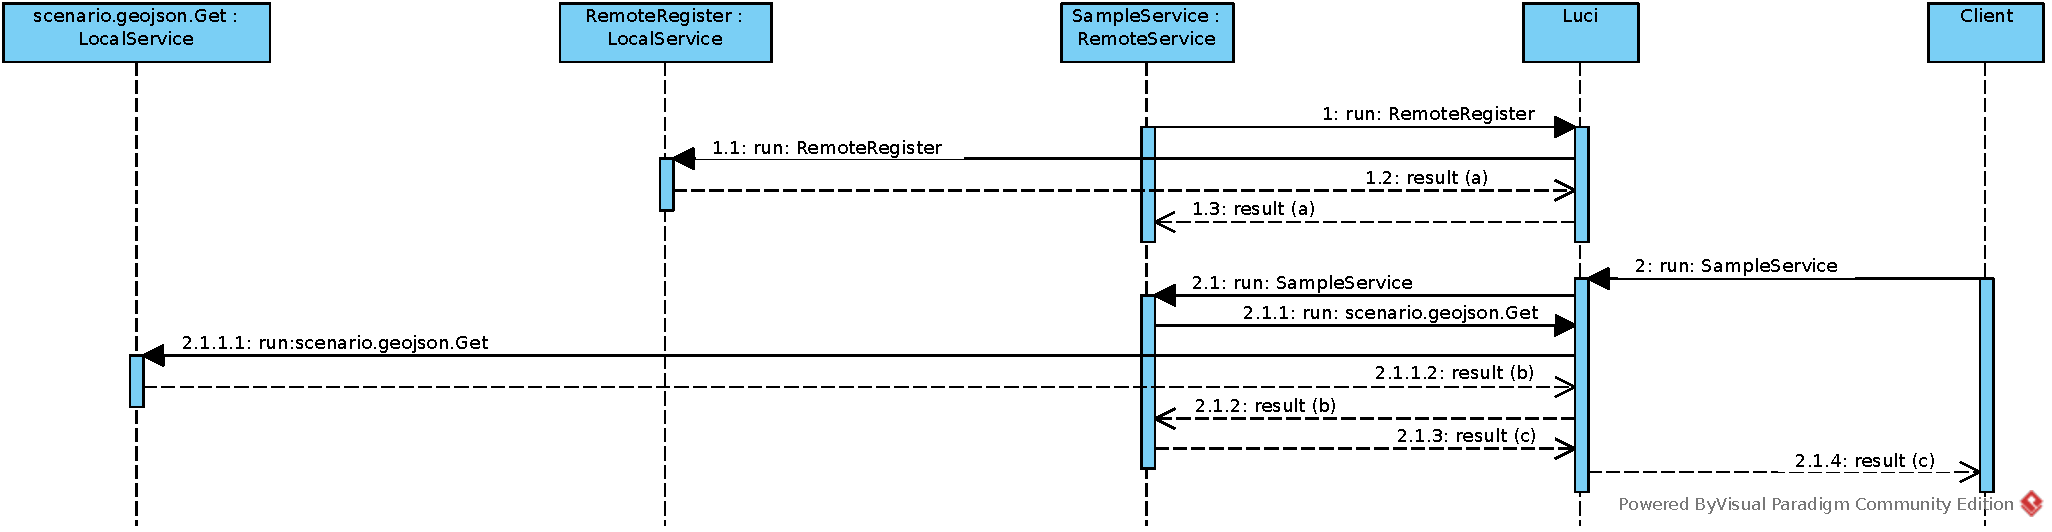
\includegraphics[width=\textwidth]{bin/assets/scenario-sequence-diagram.pdf}
	\caption{A SampleService that analyzes a scenario registers itself to Luci and is called by client as UML sequence diagram.}
\end{figure}
\vfill
\clearpage
